\documentclass[10pt]{article}
\usepackage[margin=0.72in]{geometry}
\usepackage{amsmath,amssymb,mathtools}
\usepackage{graphicx,booktabs,array,tabularx,multirow}
\usepackage{microtype,setspace}
\usepackage[numbers,sort&compress]{natbib}
\usepackage[hidelinks]{hyperref}
\usepackage{lineno}
\usepackage{xcolor}
\usepackage{caption}
\captionsetup{font=small,labelfont=bf}
\setstretch{1.02}
\newcommand{\CNS}{\mathrm{CNS}}
\newcommand{\FSS}{\mathrm{FSS}}
\newcommand{\Reg}{\operatorname{Register}}
\newcommand{\Exp}{\operatorname{Express}}
\newcommand{\Store}{\operatorname{Store}}
\newcommand{\Recall}{\operatorname{Recall}}
\newcommand{\Model}{\operatorname{Model}}
\newcommand{\Evaluate}{\operatorname{Evaluate}}
\newcommand{\Decomp}{\operatorname{Decompose}}
\newcommand{\Bridge}{\operatorname{Bridge}}
\newcommand{\Pass}{\textsc{pass}}
\newcommand{\Fail}{\textsc{fail}}
\newcommand{\Und}{\textsc{undetermined}}
\newcommand{\ModelHash}{797b16e30934}
\newcommand{\RegistryHash}{b7a6ef0e1d8c}
\newcommand{\TotalTraj}{12800}
\newcommand{\TotalEvents}{102400}
\newcommand{\NumRegimes}{160}
\newcommand{\HigherN}{816}
\newcommand{\LocalN}{464}
\newcommand{\FullHighAcc}{0.585}
\newcommand{\FullHighAccLo}{0.551}
\newcommand{\FullHighAccHi}{0.618}
\newcommand{\BestHighAcc}{0.400}
\newcommand{\BestHighAccLo}{0.366}
\newcommand{\BestHighAccHi}{0.433}
\newcommand{\FullHighReach}{0.435}
\newcommand{\FullHighReachLo}{0.401}
\newcommand{\FullHighReachHi}{0.469}
\newcommand{\BestHighReach}{0.0033}
\newcommand{\FullReuse}{0.347}
\newcommand{\FullReuseLo}{0.314}
\newcommand{\FullReuseHi}{0.379}
\newcommand{\FullLocalAcc}{0.679}
\newcommand{\BestLocalAcc}{0.595}
\newcommand{\FullContain}{0.987}
\newcommand{\IncContain}{0.717}
\newcommand{\FullHarm}{0.012}
\newcommand{\IncHarm}{0.156}
\newcommand{\FullSelect}{0.099}
\newcommand{\IncSelect}{0.366}
\newcommand{\FullOptionGain}{0.015}
\newcommand{\IncOptionGain}{0.014}
\newcommand{\FullRisk}{0.207}
\newcommand{\IncRisk}{0.266}
\newcommand{\BaseRisk}{0.320}
\newcommand{\GenericLTwo}{0.300}
\newcommand{\GenericLSixteen}{0.000}
\newcommand{\MonitorLTwo}{0.867}
\newcommand{\MonitorLEight}{0.067}
\newcommand{\MonitorFalseConfidence}{0.000}
\newcommand{\RetentionBestLoss}{0.258}
\newcommand{\RetentionIndLoss}{1.024}
\newcommand{\CodeTests}{27}
\newcommand{\CanonicalID}{0.940}
\newcommand{\CanonicalIDLo}{0.916}
\newcommand{\CanonicalIDHi}{0.958}
\newcommand{\MinCandidateID}{0.932}
\newcommand{\HeldoutDistance}{3}
\newcommand{\CompletePass}{0.856}
\newcommand{\CompletePassLo}{0.768}
\newcommand{\CompletePassHi}{0.914}
\newcommand{\ArticlePass}{0.000}
\newcommand{\NegReject}{0.711}
\newcommand{\LeakageMax}{0.481}
\newcommand{\NumWitnesses}{23}

\title{\textbf{Recursive operand closure and certified spanning generate a cognitive near-singularity}}
\author{Andy E. Williams\\
\small Nobeah Foundation, Nairobi, Kenya\\
\small Caribbean Center for Collective Intelligence, St. John's, Antigua and Barbuda\\
\small Correspondence: creative.andyewilliams@gmail.com}
\date{}

\begin{document}
\maketitle
\linenumbers

\begin{abstract}
A reasoning system can gain operations, memory or communication without gaining the ability to construct and reuse a new class of operands. We formalize a cognitive near-singularity (CNS) as recursive operand promotion combined with certified spanning of the lifted domain inside one executable, participant-indexed control system. The model couples typed non-FSS signal carriers, bidirectional transduction, a Store--Recall and local--global conceptual basis, three-dimensional current--target--projected fitness, certificates, governance and a provenance-preserving residual ledger. One event-sourced generator produced \TotalTraj\ matched synthetic trajectories and \TotalEvents\ transitions. Across \NumWitnesses\ deterministic target-pair witnesses, the complete model passed every target while each designated ablation failed or became correctly undetermined. On nonfactorizing higher-order worlds, full CNS target accuracy was \FullHighAcc\ (95\% Monte Carlo interval \FullHighAccLo--\FullHighAccHi) versus \BestHighAcc\ for the best matched comparator; certified reach was \FullHighReach\ versus \BestHighReach. Residual-closed capability preserved the participant bound in \FullContain\ of trajectories, whereas an equally capable residual-open control preserved it in \IncContain. Finite projections lost exact critical subgraphs with relational depth, and a correlation-aware retention model outperformed homogeneous independence. A \CodeTests-test signature identified the canonical reconstruction with accuracy \CanonicalID. Structural artifacts raised algorithmic reconstruction from \ArticlePass\ for Article-only to \CompletePass\ for the complete package, but the preregistered independent semantic receiver study was not executable here. Propagation closure and historical rank therefore remain undetermined.
\end{abstract}

\section*{Introduction}
Knowledge-producing systems are commonly evaluated by the number of concepts they contain, the performance of their strongest component, or the connectivity of their communication network. These quantities do not determine whether the system can construct a new operand from an admissible lower-order substructure, preserve that operand as a recoverable identity, and use it in a later globally coupled transformation. Conceptual-space and semantic-network representations make this distinction explicit: local regions can be densely developed while relations needed for a declared global target remain absent or uncertified\citep{gardenfors2000,collins1975,krenn2020}. Collective performance likewise depends on interaction topology and the preservation of diverse problem-solving routes, not only on individual ability or group size\citep{woolley2010,hong2004,lazer2007,lorenz2011}.

The same structural question arises in artificial intelligence oversight. A capable system may traverse a reasoning object larger than a human can inspect, while the evaluator receives only a finite projection. Interpretability, amplification, debate and weak-to-strong supervision each address parts of this problem\citep{murdoch2019,rudin2019,christiano2018,irving2018,burns2023}. Externally generated reasoning records can improve monitorability, but visible records remain channels whose target adequacy has to be established rather than assumed\citep{korbak2025,emmons2025}. A projection can preserve most locally salient statements and still erase one relation on which a global verdict depends.

A previously published CNS framework defined a possibility theorem for transitions between orders of conceptual traversal\citep{williams2026}. The present work asks a narrower executable question: what coupled structure is sufficient to generate an order-lifting transition, keep its consequences participant-coherent, preserve its target distinctions through bounded channels, and transmit enough evidence to distinguish the intended model from plausible reconstructions? The answer cannot be supplied by independent diagrams or module-specific simulations. If the Article, code and experiment instantiate different transition systems, apparent cross-domain agreement is not evidence for one model.

We therefore construct one event-sourced generator over a stratified conceptual functional state space (FSS), participant-indexed fitness FSSs and typed signal carriers. The generator exposes every transition through a canonical registry and residual ledger. Five linked tests form the confirmatory spine. First, designated target pairs test the necessity of boundary, conceptual and fitness functions. Second, paired worlds with identical lower-order projections test whether operand lift, global span and certification jointly generate nonfactorizing target access. Third, nested option sets test whether capability expansion has positive valence only when model, certificate, realization and participant-governance residuals are within budget. Fourth, bounded projections test exact graph recovery and false confidence as relational depth grows. Fifth, codeword experiments test whether the joint result signature identifies the canonical model and whether increasingly structural artifact packages improve reconstruction.

The experiment distinguishes three closure claims. \emph{Formal closure} means that the finite theorem and witness package has no unresolved typed contradiction within its declared targets. \emph{Execution closure} means that every reported primary result replays from one generator and one model hash. \emph{Propagation closure} means that independent competent receivers reconstruct, execute and extend an operationally equivalent model without author repair. The first two were executable in the present environment. The third required external model families and fresh independent contexts that were unavailable, so it is reported as \Und\ rather than inferred from internal consistency.

\section*{Results}

\subsection*{One generator couples boundary, conceptual and fitness functions}
This section fixes the computational object, tests whether its named functions carry distinct target contracts, and establishes the lower-order indistinguishability needed for the later CNS test.

Let the modeled FSS instances be
\begin{equation}
\mathfrak X=\{\mathcal C\}\cup\{\mathcal F_i:i\in I\},
\end{equation}
where $\mathcal C$ is the stratified conceptual space and $\mathcal F_i$ is participant $i$'s fitness space. Each $X\in\mathfrak X$ interacts through a typed carrier $\Sigma_X$, an input transducer $\Reg_X$ and an output transducer $\Exp_X$. A carrier is not an FSS: it has an encoding, source, destination, budget, delay and provenance, but no internal function basis and no recursively generated carrier boundary of its own. This type choice terminates the boundary construction while preserving bidirectional interaction (Fig.~\ref{fig:architecture}).

The conceptual internal basis contains Store, Recall, a target-local assessment $L$ and a global assessment $G$. Store preserves recoverable identity, relations, verdicts and provenance; Recall reactivates a stored object under a declared target and context budget. $L$ transforms evidence inside the represented active region. $G$ may traverse regions but must preserve all successor obligations on which the global verdict depends. Admissible composites are promoted by a Create/promotion contract to reusable higher-order operands. The fitness carrier for participant $i$ is
\begin{equation}
\mathbf f_{i,t}(a)=\left(f^{\rm cur}_{i,t},f^{\rm tar}_{i,t},f^{\rm proj}_{i,t+1\mid a}\right).
\label{eq:triad}
\end{equation}
Its three pairwise control relations generate the Model--Evaluate, Stability--Adaptation and Decomposition--Bridging dualities. Target revision is stored separately from achieved movement at a fixed target.

All these objects are coordinates of one state
\begin{equation}
Z_t=\bigl(\{X_t,\Sigma_{X,t},\Reg_{X,t},\Exp_{X,t}\}_{X\in\mathfrak X},
\Gamma_t,o_t,M_t,\{\mathbf f_{i,t},\widehat{\mathbf f}_{i,t}\}_{i\in I},\Lambda_t,e_t\bigr),
\end{equation}
updated only by
\begin{equation}
\operatorname{step}(Z_t,a_t,\xi_t)\mapsto (Z_{t+1},E_{t:t+1}),
\label{eq:step}
\end{equation}
where $\xi_t$ is a seeded stochastic input and $E_{t:t+1}$ is the append-only event batch. Every event records the model and registry hashes, operator identifier, target, resource use, residual change, seed and pre/post state hashes. Figure~\ref{fig:architecture} shows the resulting coupling. The executed model hash begins \texttt{\ModelHash}; the registry hash begins \texttt{\RegistryHash}.

\begin{figure}[t]
\centering
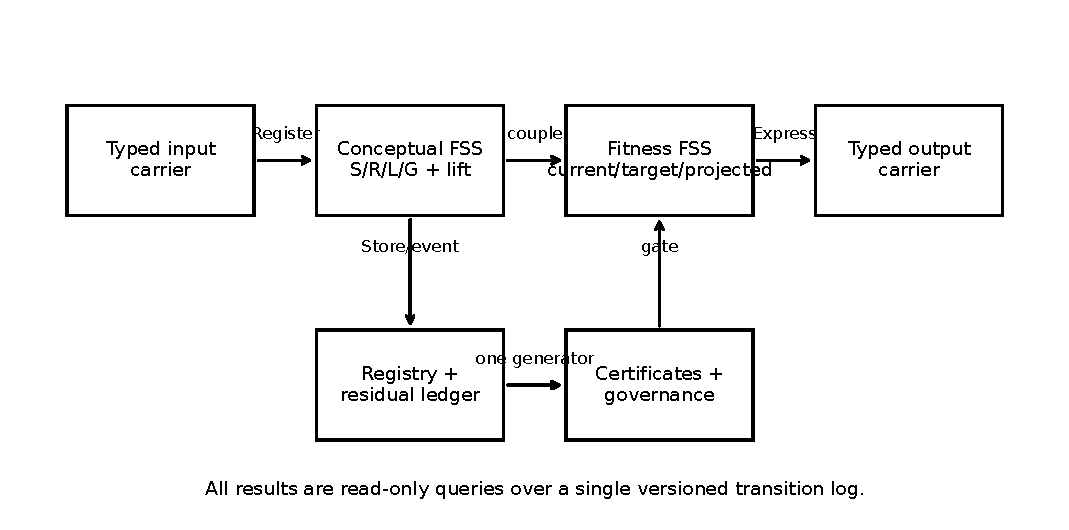
\includegraphics[width=0.96\linewidth]{../figures/fig1_architecture.pdf}
\caption{\textbf{One coupled executable object.} Typed carriers convey external structure to and from FSS instances through Register and Express. Store, Recall, local/global assessment and promotion operate in the conceptual FSS; current, target and action-conditioned projected fitness support participant-indexed control. Certificates and governance gate inter-FSS consequences. Every displayed result is a read-only query over the same event and residual ledger.}
\label{fig:architecture}
\end{figure}

The deterministic suite contained \NumWitnesses\ constructive target pairs. The complete model returned \Pass\ on all \NumWitnesses. Removing the designated contract returned \Fail\ on 16 targets and \Und\ on seven, with no ablation success (Fig.~\ref{fig:witnesses}; Supplementary Table~4). The distinction matters: for targets requiring an unavailable higher-order distinction, an ablation should abstain rather than fabricate a verdict. Type-erasing a signal carrier, omitting Store provenance, collapsing Store into Recall, reversing Register and Express, dropping a fitness coordinate, accepting a false bridge, aggregating away one participant, counting target movement as improvement, and replacing the generator with a locally fitted surrogate each changed at least one designated verdict.

Equation~\ref{eq:triad} was tested with paired control instances. For each omitted coordinate, the remaining two coordinates were identical while the required action was opposite. Every two-coordinate controller was therefore exactly 0.500 accurate on its designated pair; the full triple was 1.000 accurate. This is a constructive minimality result for the declared controller, not a claim that every control problem has three Euclidean coordinates.

The order-lift test used 10,000 paired worlds whose complete lower-order feature vectors occurred with both higher-order labels. Logistic regression and an unconstrained random forest obtained at most \LeakageMax\ held-out accuracy. The paired construction therefore supplied no usable lower-order leakage before the integrated comparison.

\begin{figure}[t]
\centering
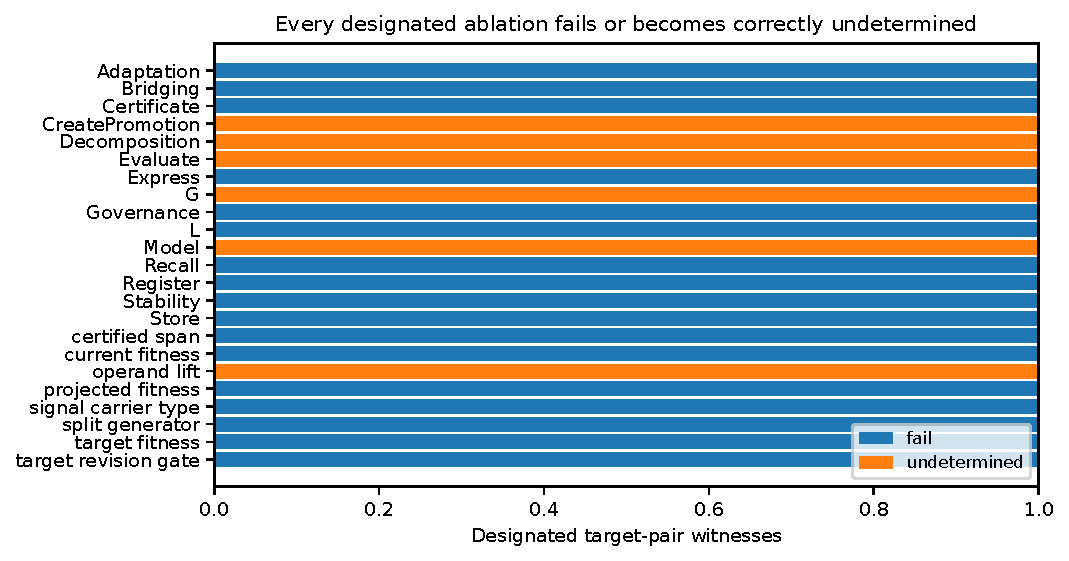
\includegraphics[width=0.96\linewidth]{../figures/fig2_witnesses.pdf}
\caption{\textbf{Function and type necessity in the declared witness family.} The complete model passed every target. Each designated ablation either failed the target or returned the typed verdict undetermined. No target was rescued by a hidden persistence index, external evaluator label, cached identity or module-local transition.}
\label{fig:witnesses}
\end{figure}

\subsection*{Operand lift, certified span and recovery generate a nonfactorizing transition}
This section asks whether additional compute, memory, population or communication can reproduce the target access created by recursive promotion plus certified global span.

The conceptual hierarchy is predicative. Level one contains grounded nodes and typed relations; for $n\geq1$,
\begin{equation}
X_{n+1}=\{\rho_n(A):A\in\operatorname{AdmSub}_n(X_{\leq n})\},
\end{equation}
where $\rho_n$ is the registered Create/promotion operation and type maps are strictly level-raising. Each paired world $(W^0,W^1)$ satisfies
\begin{equation}
q_n(W^0)=q_n(W^1),\qquad \Phi_{n+1}(W^0)\neq\Phi_{n+1}(W^1).
\label{eq:nonfactor}
\end{equation}
A successful trajectory must admit the grounded signal, construct the admissible composite, validate and Store it, Recall it as an operand, connect it to the target through a certified path, and Express the verdict. Nominal connectivity without certificate fidelity is recorded separately from certified reach.

We generated 128 scrambled Sobol regimes and 32 preregistered corner regimes over bridge difficulty, certificate noise, Store/Recall noise, boundary noise, model and evaluation residuals, governance conflict, hazard, realization fidelity, option cost, context demand and target drift. Each regime received eight common-random-number replicates under ten patches to the same generator: local baseline, matched compute, memory, population and communication, certification-only, lift-only, span-only, full CNS and an equally capable residual-open CNS. This produced \TotalTraj\ trajectories, including \HigherN\ higher-order and \LocalN\ local-target observations per intervention.

On higher-order targets, full CNS externally expressed the correct verdict in \FullHighAcc\ of trajectories (95\% Monte Carlo interval \FullHighAccLo--\FullHighAccHi). The best matched comparator, increased communication, reached \BestHighAcc\ (\BestHighAccLo--\BestHighAccHi). Full certified reach was \FullHighReach\ (\FullHighReachLo--\FullHighReachHi), compared with \BestHighReach\ for the best non-CNS comparator, and recursive reuse occurred in \FullReuse\ (\FullReuseLo--\FullReuseHi). Lift-only and span-only produced zero certified reach because each lacked the other factor; certification-only could validate the rare local nominal path but could not create the missing operand (Fig.~\ref{fig:cns}). The residual-open capability control attained intermediate nominal capability but lost certificate and boundary fidelity.

The result was target-conditional rather than a generic performance bonus. In worlds without a higher-order target, full CNS accuracy was \FullLocalAcc\ and matched compute accuracy was \BestLocalAcc; the absolute advantage contracted from 0.185 on the paired higher-order family to 0.084. The remaining local difference reflects boundary, Store/Recall and certificate improvements bundled into the full patch. No claim is made that recursive promotion dominates a comparator whose existing resources can enumerate the complete target.

\begin{figure}[t]
\centering
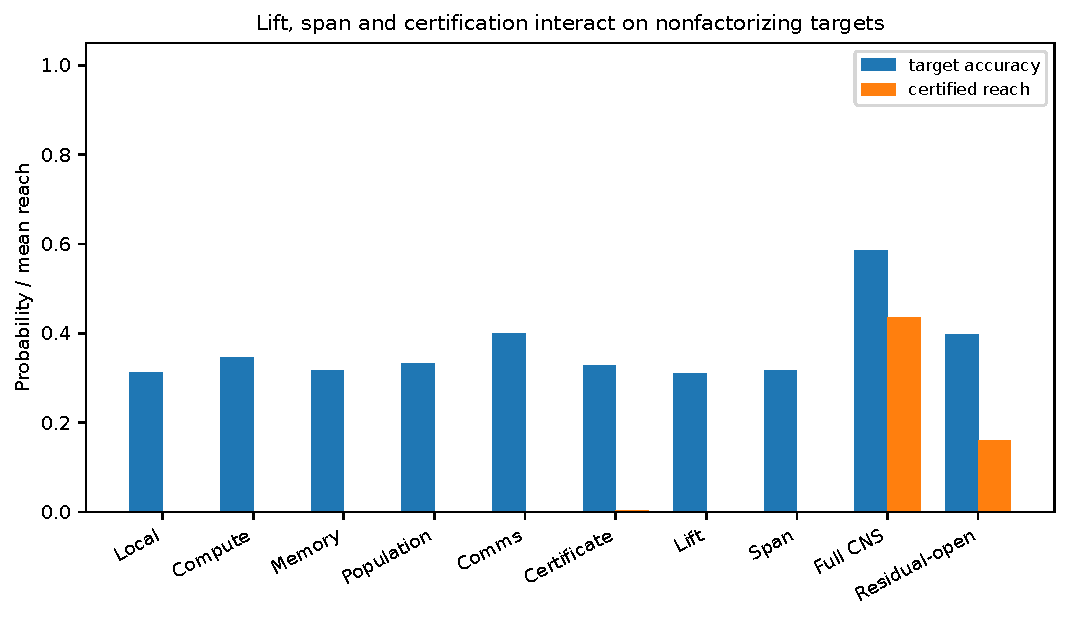
\includegraphics[width=0.98\linewidth]{../figures/fig3_cns_transition.pdf}
\caption{\textbf{Nonfactorizing capability transition.} Bars show target accuracy and certified reach on higher-order worlds. Resource increases, lift alone, span alone and certification alone do not reproduce the conjunction. The residual-open control has the same nominal capability family as the full CNS but lower certificate, boundary and governance fidelity. Intervals and full numeric results are in Supplementary Table~5.}
\label{fig:cns}
\end{figure}

\subsection*{Global coherence conditions the valence of capability expansion}
This section keeps the capability superset fixed while varying whether its participant consequences, certificates, signals and target revisions are inside the declared residual budget.

Each world supplied a baseline option set $O_b$ and a CNS superset $O_a\supseteq O_b$. For participant $i$, the generator represented the current state, target and action-conditioned successor, then selected an action using the stored governance rule. Let represented and realized utility at the fixed target differ by at most $\epsilon_i$, and let selection error be at most $\delta_i$. If the admissibility and governance gate retains every baseline option and chooses the new option only when every represented participant outcome clears the lower confidence bound, then the selected action $a^*$ satisfies the finite option bound
\begin{equation}
u_i(a^*)\geq \max_{b\in O_b}u_i(b)-(2\epsilon_i+\delta_i)
\label{eq:option}
\end{equation}
for every governed participant. The experiment implemented Eq.~\ref{eq:option} directly. It also generated negative controls with aggregate governance, stale projections, false certificates, lossy realization and ungoverned target shift.

The residual-closed CNS selected the new option in \FullSelect\ of trajectories and improved mean participant outcome relative to the retained baseline by \FullOptionGain. It remained inside the preregistered $-0.03$ participant bound in \FullContain\ of trajectories. The fraction of participant-action outcomes strictly below baseline was \FullHarm; these small losses were concentrated near the bound and arose from stochastic realization. The residual-open control selected the new option in \IncSelect\, achieved a similar mean gain (\IncOptionGain), but participant-bound containment fell to \IncContain\ and the harmed participant-action fraction rose to \IncHarm\ (Fig.~\ref{fig:coherence}). Thus the mean did not identify valence: the same average improvement coexisted with materially different participant tails.

The survival view was derived from the same terminal consequences, not assigned by the CNS label. Under the preregistered synthetic hazard bridge, terminal-risk frequency was \FullRisk\ for the residual-closed CNS, \IncRisk\ for the residual-open control and \BaseRisk\ for the local baseline. These are model-internal projections, not estimates of civilization-level risk. Positive, neutral and negative CNS effects remain possible when the hazard, realization or governance bridges change.

\begin{figure}[t]
\centering
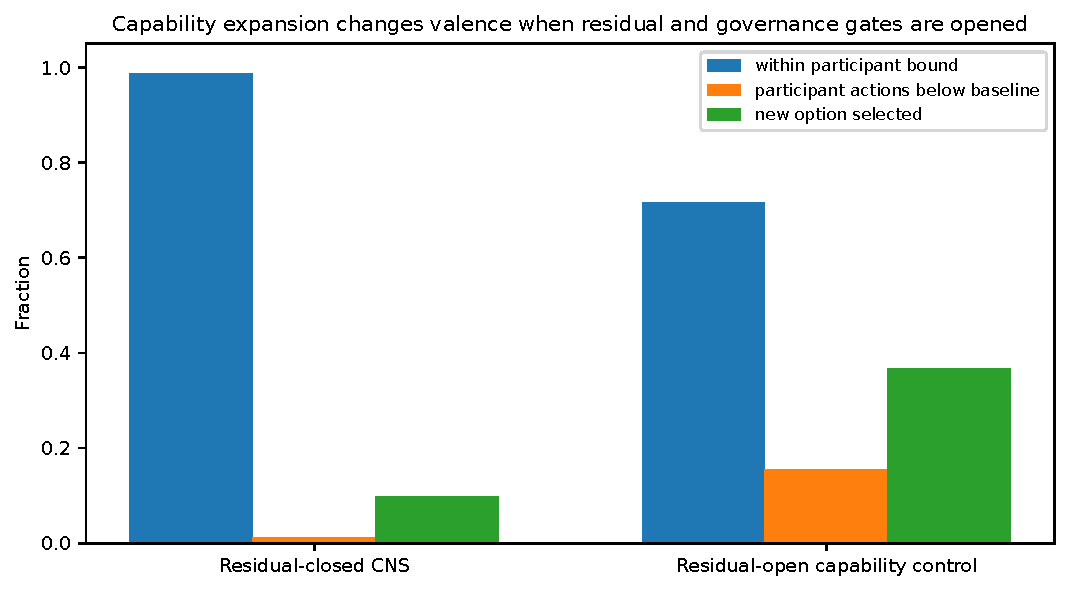
\includegraphics[width=0.96\linewidth]{../figures/fig4_coherence.pdf}
\caption{\textbf{Coherence-conditioned option expansion.} The residual-closed and residual-open conditions use the same lifted capability family. Bars report the fraction of trajectories satisfying the participant bound, the participant-action fraction below the retained baseline, and the frequency with which a new option was selected. Mean improvement alone does not distinguish the two regimes.}
\label{fig:coherence}
\end{figure}

\subsection*{Bounded projections lose exact target structure with relational depth}
This section tests the observability implication of the same model: a target verdict is checkable only if the visible projection preserves every distinction on which it depends.

Let $X$ be a complete target-relevant state, $q:X\rightarrow Z$ a finite visible projection and $\Phi:X\rightarrow\{0,1\}$ a target predicate. Exact adequacy requires
\begin{equation}
q(x)=q(y)\Longrightarrow \Phi(x)=\Phi(y),
\label{eq:adequacy}
\end{equation}
or equivalently $\Phi=f\circ q$ for some decoder $f$. When $L$ critical relations are conjunctively required and relation retention is homogeneous and conditionally independent, exact recovery is $q^L$. Real records can contain heterogeneous relations, redundancy and correlated pipeline quality, so this law is a null model rather than a universal prediction.

The bounded-registration suite generated three synthetic trace families, relation depth $L\in\{2,4,6,8,12,16\}$, budgets $K\in\{128,256,512,1024\}$, redundancy $r\in\{1,2,4\}$ and three projection pipelines: generic summary, fixed-budget relation extraction and a target-aware three-valued monitor. Thirty independent tasks were produced per cell. At $K=256$ and $r=1$, generic-summary exact recovery declined from \GenericLTwo\ at $L=2$ to \GenericLSixteen\ at $L=16$. The target-aware monitor improved recovery to \MonitorLTwo\ at $L=2$ and \MonitorLEight\ at $L=8$, while holding false confidence at \MonitorFalseConfidence\ by returning undetermined when the critical subgraph was incomplete (Fig.~\ref{fig:observation}).

A preregistered correlation-aware logistic retention model had held-out log loss \RetentionBestLoss, compared with \RetentionIndLoss\ for homogeneous independence. Performance above $q^L$ therefore rejected the homogeneous null but did not remove the bounded-registration target: exact recovery still depended strongly on depth, capacity, redundancy and projection class. The planned external trace experiment across three version-locked language-model families could not be collected in the available environment. The present result is consequently a synthetic mechanism and analysis protocol, not evidence about the completeness of any current model's internal reasoning.

\begin{figure}[t]
\centering
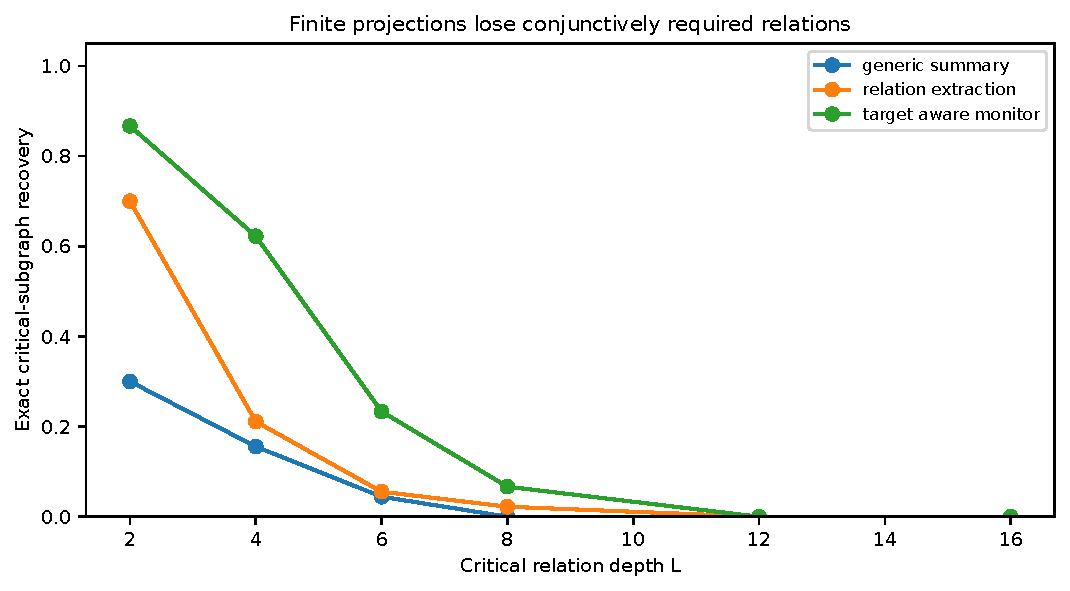
\includegraphics[width=0.96\linewidth]{../figures/fig5_observability.pdf}
\caption{\textbf{Exact recovery under bounded registration.} Curves average three synthetic trace families at budget $K=256$ and redundancy one. Generic summaries retain many individual relations at small depth but rapidly lose the complete critical subgraph. A target-aware three-valued monitor increases exact recovery and prevents false confidence by abstaining when the target does not factor through the record.}
\label{fig:observation}
\end{figure}

\subsection*{The joint signature identifies the model, but semantic propagation remains undetermined}
This section separates experimental identification of the executable model from independent reconstruction of that model by a receiver.

We preregistered the canonical model $M^*$ and 12 target-different reconstructions: signal-less input, recursive signal-FSS regress, Store/Recall collapse, verdict-only or connectivity-only global assessment, primitive promotion, two-coordinate fitness variants, aggregate governance, uncertified reach, split generators and target-shift value. For a test set $Q=\{q_1,\ldots,q_K\}$, each model predicts a codeword
\begin{equation}
\mathbf y(M_j)=\bigl(q_1(M_j),\ldots,q_K(M_j)\bigr).
\end{equation}
A greedy plus local-search selector retained \CodeTests\ tests spanning every causal layer and increased the minimum candidate distance. With 1.5\% independent observation flips, nearest-valid-codeword decoding identified $M^*$ in \CanonicalID\ of 500 runs (Wilson 95\% interval \CanonicalIDLo--\CanonicalIDHi); the lowest candidate accuracy was \MinCandidateID. Eight held-out contract recombinations had minimum distance \HeldoutDistance\ from the canonical selected codeword.

The transmitted package was then ablated into Article-only, Article plus Supplement, registry, code/tests and complete structural conditions. Three explicitly algorithmic receiver classes -- lexical, schema-first and conformance-driven parsers -- attempted standardized contract recovery, held-out prediction and an extension adapter. Their mean pass rate rose from \ArticlePass\ under Article-only to \CompletePass\ under the complete package (Wilson interval \CompletePassLo--\CompletePassHi; Fig.~\ref{fig:propagation}). A fluent negative-control package containing one contract inversion was rejected in \NegReject\ of runs, showing residual room for improvement.

This stress test establishes machine readability of the supplied artifacts; it does not satisfy the preregistered propagation criterion. The plan required at least three independent external language-model families in fresh contexts, a lower confidence bound above 0.80, at least 95\% deterministic held-out prediction, 90\% unseen-extension success and no systematic fatal inversion. The pooled surrogate lower bound was \CompletePassLo, and the receiver algorithms were authored with knowledge of the artifact format. Propagation closure is therefore \Und. This negative status is a result of the declared conjunction rule, not an editorial caveat that can be averaged away.

\begin{figure}[t]
\centering
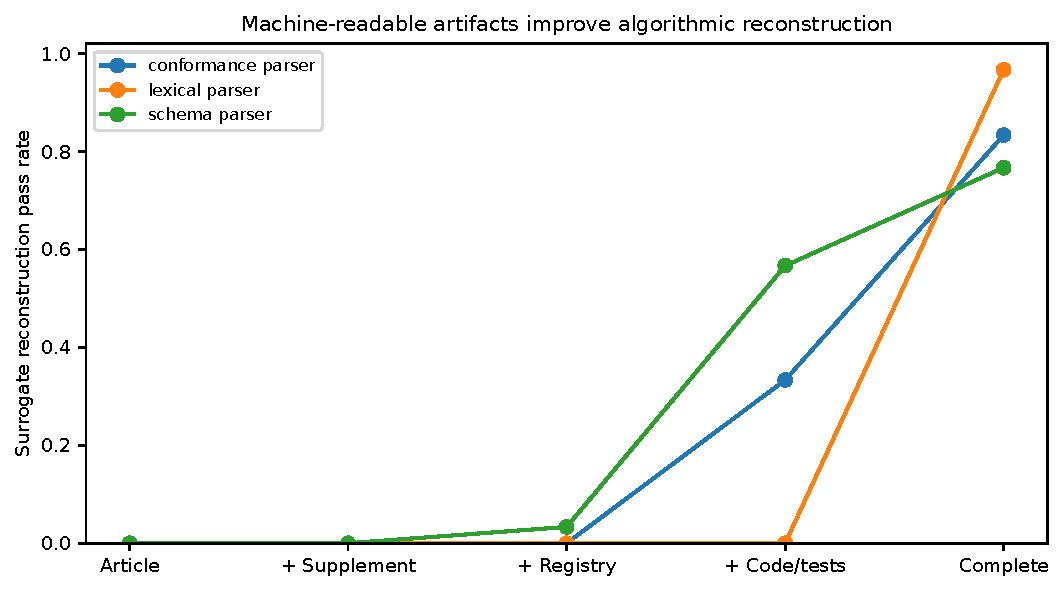
\includegraphics[width=0.96\linewidth]{../figures/fig6_propagation.pdf}
\caption{\textbf{Artifact layers and algorithmic reconstruction.} Three parser families received nested packages. Structural registry and conformance artifacts sharply increased exact contract recovery and executable extension. Because these parsers are not independent semantic receiver models, the figure is a transmission stress test rather than a propagation-closure result.}
\label{fig:propagation}
\end{figure}

\section*{Discussion}
The experiment supplies a constructive computational witness for one coupled claim. A reasoning system crosses the declared CNS boundary when it can promote an admissible lower-order substructure to a reusable operand and reliably span the lifted domain, while grounded input, recoverable memory, certification, participant-indexed control and output realization remain inside target-relative residual budgets. More compute, memory, participants or communication do not reproduce this transition when their operator image excludes the higher-order distinction. Conversely, lift without span and span without lift each remain insufficient.

The single-generator requirement is scientifically load-bearing. A conceptual theorem, a control simulation and a propagation benchmark can be made mutually suggestive while silently using different state transitions. Here all \TotalEvents\ transitions carry one model hash, all summaries are derived from the same event log, and deterministic replay reproduced a selected trajectory's complete post-state hash sequence. The split-generator negative model was distinguishable in the selected codeword. This does not establish that the canonical model is the only useful description of cognition. It establishes that the reported projections belong to one exhibited computational object rather than a collection of analogies.

The fitness result also narrows the meaning of positive importance. A capability superset can retain every baseline option, yet become harmful when the system mis-models consequences, validates a false bridge, loses a signal during realization, changes the target without authorization or aggregates away one participant. Participant-complete lower-confidence selection converted the option-set inclusion into a finite displacement bound. Opening the same residual and governance gates preserved the mean while worsening participant tails. Importance is therefore a participant-indexed displacement object with target revision kept separate, not an intrinsic scalar attached to capability.

Bounded observability connects the computational object to oversight without assuming hidden intent. Exact evaluation fails whenever the target does not factor through the visible projection. Correlation and redundancy alter the simple $q^L$ law; the experiment confirms that they can improve recovery substantially. They do not make finite capacity irrelevant. A target-aware monitor can also improve safety by returning undetermined rather than issuing a confident verdict from an incomplete graph. Empirical evaluation should therefore report exact critical-subgraph recovery, abstention calibration and false confidence, not only average relation retention.

The strongest planned claim -- propagation closure -- was not reached. The complete package substantially improved three algorithmic reconstructions, but those receivers were not independent language-model families and the pooled lower confidence bound missed the preregistered 0.80 threshold. The unexecuted external trace and historical audits similarly prevent claims about current AI internals or civilization's highest-importance innovation. The status-conditioned title is consequently the plan's Status~3 title: it states the synthetic mechanism rather than historical maximality.

Several limitations define the scope. The worlds are generated to isolate declared contracts; their parameter distribution is not measured from human institutions or deployed AI. The deterministic witnesses demonstrate irreducibility only for the stated target family and resource exclusions. The candidate reconstruction library is finite, and held-out variants were algorithmically generated rather than supplied by independent reviewers. The residual and hazard bridges are synthetic. The three-dimensional fitness carrier presupposes a valid order embedding for each target; non-embeddable partial orders must remain partial and return undetermined rather than be scalarized. Finally, the Article and Supplement have not themselves passed the independent no-author-repair receiver study that the theory identifies as the terminal transmission test.

The next experiment is therefore concrete. Freeze the present package, collect externally available reasoning records from at least three version-locked model families on the declared relational tasks, and assign the five nested artifact packages plus the negative control to independent receiver families with browsing disabled and fresh contexts. The secret extension target should be generated only after package freeze. A successful result would close a different theorem target from the synthetic benchmark: not merely that one author can implement the model, but that the public artifacts regenerate an operationally equivalent model in independent receivers.

\section*{Methods}

\subsection*{Canonical registry, state and transition order}
The registry contains 15 load-bearing function contracts: Register, Express, Store, Recall, $L$, $G$, Create/promotion, Model, Evaluate, Stability, Adaptation, Decomposition, Bridging, Certificate and Governance. Aliases map presentation-specific names to these identifiers. Two inherited obligations are stored explicitly: R1 records the prior omission of Store from an inventory; R2 leaves Destroy bounded-open unless a target pair requires it independently of registered composites. Local inventories and figure labels are generated from the registry.

Each trajectory executes eight ordered phases through Eq.~\ref{eq:step}: Register; Recall/activation; local or global assessment with optional lift/span construction; certificate validation; participant modeling, evaluation and governance; Store and recursive reuse; target verdict plus Express; and realization. Parallel implementations may reorder independent instructions but may not change this dependency relation. The event schema records trajectory identifier, event index, operator, model and registry hashes, pre/post state hashes, target, resource and residual deltas, world, intervention and seed.

\subsection*{Deterministic witnesses and hidden-resource audit}
Each function received a constructive target pair in which the complete contract resolves a distinction and the designated ablation lacks it. Ablations were prohibited from recovering the missing contract through preprocessing, labels, cached identity, external indexing or a special-case world generator. The hidden-resource audit inserted forbidden support into test fixtures and verified that the conformance suite detected the dependency. Metamorphic checks covered admissible renaming, graph relabeling, order-preserving fitness transformations and deterministic replay. Type erasure, contract inversion, false certificates, dropped provenance and split generators were required to alter at least one verdict.

For the fitness triad, three paired families held two coordinates fixed and varied the third so that the optimal action reversed. The best deterministic rule over the retained coordinates is therefore 0.5 accurate on each designated pair. The full rule uses all three coordinates and is exact by construction.

\subsection*{Nonfactorizing worlds and interventions}
Lower-order feature vectors contained 12 binary coordinates. Each vector occurred twice with opposite higher-order labels, then the 10,000 records were shuffled. Leakage was assessed using logistic regression and a 200-tree random forest on a stratified held-out split.

The integrated generator used 128 scrambled Sobol regimes and 32 corner regimes. Continuous coordinates controlled higher-order prevalence, bridge difficulty, certificate, Store, Recall and boundary noise, model and evaluation residuals, governance conflict, hazard, realization fidelity, option cost, context demand and target drift. A higher-order target was present when the first coordinate exceeded 0.30. Every regime was run with eight common-random-number replicates for each of ten intervention patches. Patches modified registry-enabled functions or resources; they did not fork the transition function. Resource counters recorded compute, memory, communication, validation and operation counts.

Target accuracy required a correct internally generated verdict and successful Express. Certified reach required a nominal path and a valid certificate. Recursive reuse required an admissibly promoted object that was Stored and later Recalled. Local-target worlds permitted direct local evidence; higher-order paired worlds did not.

\subsection*{Participant option and hazard construction}
Each trajectory contained 16 participants. Current fitness was sampled uniformly, targets were positive offsets, and the retained baseline action produced a modest stochastic improvement. A candidate CNS option had a larger expected gain in low-conflict worlds. High-conflict worlds introduced participant-specific negative consequences. The full CNS formed an action-conditioned realization estimate and selected the new option only if every participant's lower confidence margin exceeded the baseline, viability held, the certificate was valid and the boundary residual was within budget. The residual-open control used aggregate mean support and nominal reach.

Achieved displacement was computed at the fixed stored target. Target revision was logged separately and was not added to displacement. Participant containment allowed a tolerance of $-0.03$ relative to the retained baseline. The terminal-risk view sampled a preregistered synthetic hazard from regime intensity, maximum unresolved residual, failed target verdict and realization fidelity. This view is a read-only projection of generated consequences.

\subsection*{Bounded-registration suite}
The suite crossed six relation depths, four equivalent field budgets, three redundancy levels, three projection pipelines and three synthetic trace families, with 30 independent tasks per cell. A record-level latent quality term induced correlated retention. Redundant expressions survived if at least one instance was retained, subject to the shared capacity budget. Generic and relation-extraction pipelines could issue a valid verdict from an incomplete subgraph, generating false confidence. The target-aware monitor returned valid only after exact recovery and otherwise returned undetermined.

Five candidate retention families were specified in the revision plan. The executable comparison reported here includes homogeneous independence, heterogeneous independence and a correlation-aware logistic model with family, projection, depth, log budget and log redundancy. Models were compared on a deterministic 20\% task holdout using log loss and Brier score.

\subsection*{Codeword identification and artifact stress test}
The candidate library included $M^*$ and 12 target-different models. A pool of 27 deterministic compound tests was generated from the registry. Selection began with at least one test from each causal layer, then greedily maximized the number of unique codewords and minimum Hamming distance. Noise-aware identification flipped each selected bit independently with probability 0.015 and decoded to the nearest valid codeword over 500 runs per candidate. Eight held-out models were generated after test selection by recombining one to three contracts, rejecting duplicates and variants closer than three selected bits to $M^*$.

The artifact stress test used six package conditions and three parser families with 30 runs per cell. Required outputs were exact mandatory-contract recovery, at least 95\% deterministic prediction, unseen-extension success and rejection of a fatal inversion. Wilson intervals were used for binary package pass rates\citep{wilson1927}. Because the parser families and error model were implemented inside the same package, this experiment was labelled a surrogate and excluded from the propagation-closure verdict.

\subsection*{Uncertainty, reproducibility and status rule}
The master seed was 20260715. The runtime-only pilot fixed 128 Sobol plus 32 corner regimes and eight replicates before the final labelled output was inspected. Primary stochastic intervals are mean $\pm1.96$ Monte Carlo standard errors clipped to the observed support. Binary receiver and identification intervals are Wilson intervals. These quantify simulation and reconstruction-run uncertainty under the stated generator, not population uncertainty.

The conformance suite verifies unique registry identifiers, stored R1/R2 obligations, non-FSS carrier typing, one model and registry hash, eight events per trajectory, deterministic replay, summary equality, no ablation pass, and detection of signal-regress and split-generator codewords. Computational research practices follow executable-manifest and rebuild principles\citep{sandve2013}. The propagation verdict is conjunctive: a high average score cannot compensate for a fatal contract inversion or an unexecuted independent receiver test.

\section*{Data availability}
All data are synthetic. The complete compressed trajectory table, event log, bounded-observation records, codewords, held-out variants and source data for every figure are included in the accompanying computational package under \texttt{data/}. A permanent public repository DOI should replace the submission-package location before publication.

\section*{Code availability}
The complete generator, registry, schemas, frozen configuration, figure builder and conformance suite are included in the accompanying package. Running \texttt{python run\_experiment.py} rebuilds the synthetic results and figures; \texttt{python tests/test\_conformance.py} executes replay and type checks. Dependency versions are frozen in \texttt{requirements.txt}.

\section*{Acknowledgements}
The author used an AI language model for drafting assistance and code generation. The author reviewed the model assumptions, executable code, generated results, references and final claims and is responsible for the work.

\section*{Author contributions}
A.E.W. conceived the study, defined the theoretical framework, designed the experiment, evaluated the implementation, interpreted the results and prepared the manuscript.

\section*{Competing interests}
The author declares no competing interests.

\bibliographystyle{unsrtnat}
\bibliography{nature_v8}
\end{document}
